% coding:utf-8

%----------------------------------------
%FOSAMATH, a LaTeX-Code for a mathematical summary for basic analysis
%Copyright (C) 2013, Daniel Winz, Ervin Mazlagic, Adrian Imboden, Philipp Langer

%This program is free software; you can redistribute it and/or
%modify it under the terms of the GNU General Public License
%as published by the Free Software Foundation; either version 2
%of the License, or (at your option) any later version.

%This program is distributed in the hope that it will be useful,
%but WITHOUT ANY WARRANTY; without even the implied warranty of
%MERCHANTABILITY or FITNESS FOR A PARTICULAR PURPOSE.  See the
%GNU General Public License for more details.
%----------------------------------------

% coding:utf-8
\section{Rechenregeln}
\subsection{Bruchrechnen}
\[ \boxed{\frac{a}{b} \cdot \frac{c}{d} = \frac{a \cdot c}{b \cdot d}} \]
\[ \boxed{n \frac{a}{b} = \frac{n \cdot a}{b}} \]
\[ \boxed{\frac{a}{b} : \frac{c}{d} = \frac{a}{b} \cdot \frac{d}{c} 
= \frac{a \cdot d}{b \cdot c}} \]

\subsection{Polynomdivision}
Das Vorgehen bei der Polynomdivision ist identisch zur schriftlichen 
Division. \\\\
Beispiel: 
% \[ \boxed{\begin{array}{rrrlrl}
% &(9x^3 &- 6&x^2 &- 8x&):(3x + 4) = \underline{\underline{3x^2 + 2x}}\\
% -&(9x^3 &- 12&x^2)&&\\
% &&6&x^2 &- 8x&\\
% &&-(6&x^2 &- 8x&)\\
% &&&&0&
% \end{array}} \]

\begin{tabular}{|r@{}r@{}r@{}r@{}l@{}r@{}r@{}l|}
\hline
\rule{0pt}{12pt}&&$(9x^3 $&$- 6$&$x^2 $&$- 8x$&$)$&$:(3x + 4) 
= \underline{\underline{3x^2 + 2x}}$\\
&$-$&$(9x^3 $&$- 12$&$x^2)$&$\downarrow\,\,$&&\\
\cline{2-5}\rule{0pt}{12pt}&&&$6$&$x^2 $&$- 8x$&&\\
&&&$-(6$&$x^2 $&$- 8x$&$)$&\\
\cline{4-7}\rule{0pt}{12pt}&&&&&$0$&&\\
\hline
\end{tabular}


\subsection{Potenzen}
\[ \boxed{a^n = a \cdot a^{n-1} \quad a^1 = a} \]
\[ \boxed{a^0 = 1 \quad \left(0^0\right)\text{ ist nicht definiert}} \]
\[ \boxed{a^{-1} = \frac{1}{a}} \]
\[ \boxed{a^{-n} = \frac{1}{a^n}} \]

\subsection{Potenzgesetze}
\[ \boxed{a^x \cdot a^y = a^{x+y}} \]
\[ \boxed{\frac{a^x}{a^y} = a^{x-y}} \]
\[ \boxed{(a^x)^y = a^{xy}} \]
\[ \boxed{a^x \cdot b^x = \left(ab\right)^x} \]
\[ \boxed{\frac{a^x}{b^x} = \left(\frac{a}{b}\right)^x} \]
\[ \boxed{a^{\frac{p}{q}} = \sqrt[q]{a^p}} \]

\subsection{Wurzeln}
\[ \boxed{\sqrt[n]{a^m} = a^{\frac{m}{n}} \quad \left(a>0; m, n \in \mathbb{N}; 
m \geq 1; n \geq 2\right)} \]
\[ \boxed{\sqrt[n]{1}=1 \quad \sqrt[n]{0}=0 \quad \sqrt[n]{a^n}=a 
\quad \left(a>0\right)} \]

\subsection{Wurzelgesetze}
\[ \boxed{\sqrt[n]{a}\cdot \sqrt[n]{b}=\sqrt[n]{a\cdot b}} \]
\[ \boxed{\frac{\sqrt[n]{a}}{\sqrt[n]{b}}=\sqrt[n]{\frac{a}{b}}} \]
\[ \boxed{\left(\sqrt[n]{a}\right)^k=\sqrt[n]{a^k}} \]
\[ \boxed{\sqrt[nk]{a^{mk}}=\sqrt[n]{a^m}} \]
\[ \boxed{\sqrt[n]{\sqrt[m]{a}}=\sqrt[m]{\sqrt[n]{a}}=\sqrt[mn]{a}} \]

\subsection{Logarithmengesetze}
\[ \boxed{y=\log_ax \Leftrightarrow a^y=x} \]
\[ \boxed{\log_a1=0 \quad \log_aa=1} \]
\[ \boxed{\lg a=\log_{10}a \quad \ln a = \log_ea} \]
\[ \boxed{a^{\log_ax}=x} \]
\[ \boxed{\log_a\left(a^x\right)=x} \]
% \subsubsection{Produkte}
\[ \boxed{\log_b\left(x \cdot y\right) 
= \log_b\left(x\right) + \log_b\left(y\right)} \]
% \subsubsection{Quotienten}
\[ \boxed{\log_b \left( \frac{x}{y} \right) 
= \log_b\left(x\right) - \log_b\left(y\right)} \]
% \subsubsection{Summen und Differenzen}
%\[ \boxed{\log_b\left(x \cdot y\right) 
% = \log_b\left(x\right) + \log_b\left(y\right)} \]
\[ \boxed{\log_b\left(x + y\right) 
= \log_b\left(x\right) + \log_b\left(1 + \frac{y}{x}\right)} \]
% \subsubsection{Potenzen}
\[ \boxed{\log_b\left(x^r\right) = r \cdot \log_b\left(x\right)} \]
\[ \boxed{\log_ax=\frac{\lg x}{\lg a}=\frac{\ln x}{\ln a}} \]

\newpage
\subsection{Trigonometrie}

\begin{figure}[h!]
\centering
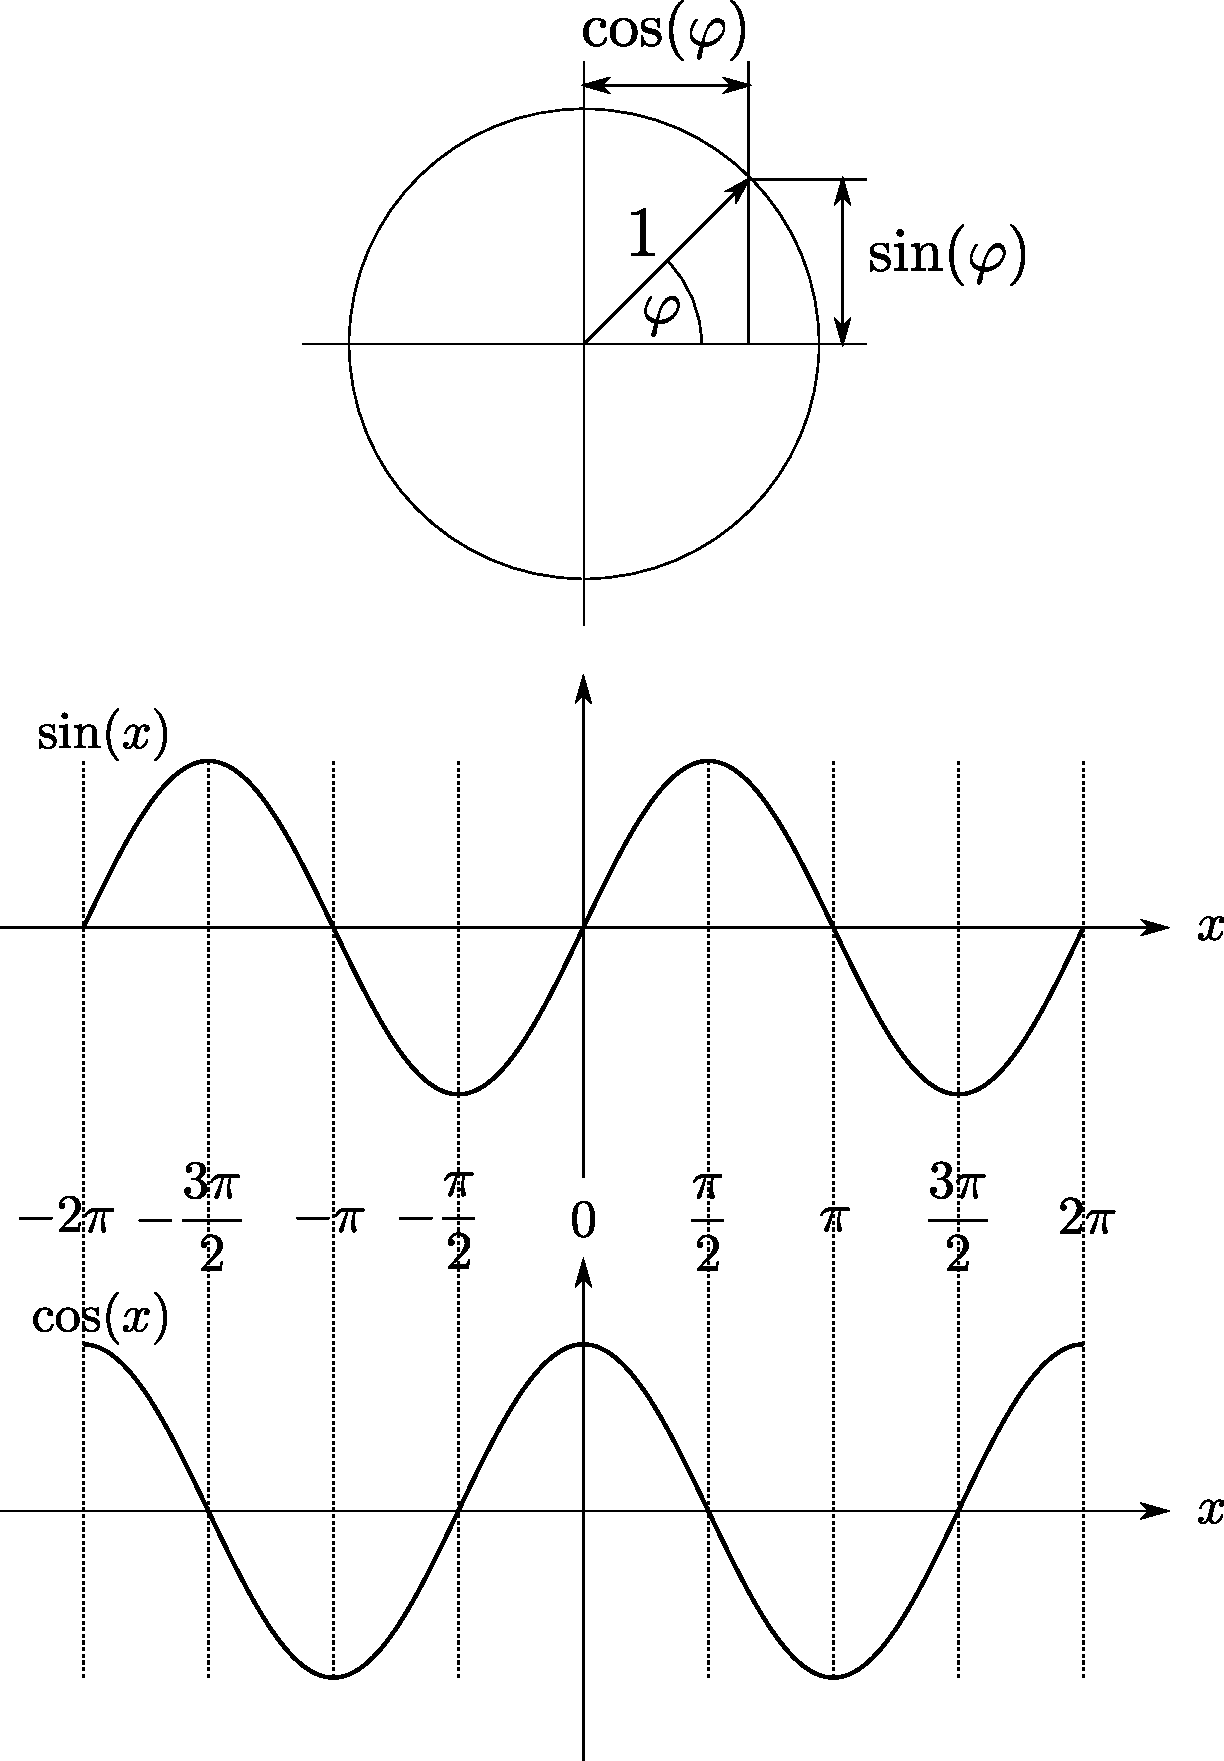
\includegraphics[width=0.8\textwidth]{einheitskreis.pdf}
\end{figure}

% \newpage
\noindent
$H$: Hypotenuse\\
$A$: Ankathete\\
$G$: Gegenkathete
\[ \boxed{\sin\alpha=\frac{G}{H}} \quad \boxed{\cos\alpha=\frac{A}{H}} 
\quad \boxed{\tan\alpha=\frac{G}{A}} \quad \boxed{\cot\alpha=\frac{A}{G}} \]
\[ \boxed{\sin x = \sqrt{1-\cos^2x} = \sqrt{\frac{\tan^2x}{1+\tan^2x}}} \]
\[ \boxed{\cos x = \sqrt{1-\sin^2x} = \sqrt{\frac{1}{1+\tan^2x}}} \]
\[ \boxed{\tan x = \frac{\sin x}{\sqrt{1-\sin^2x}} 
= \frac{\sqrt{1-\cos^2x}}{\cos x} = \frac{\sin x}{\cos x}} \]
\[ \boxed{\sin^2 x + \cos^2 x = 1} \]

\subsubsection{Additionstheoreme}
\[ \boxed{\sin(x+y) = \sin(x) \cdot cos(y) + \cos(x) \cdot \sin(y) }\]
\[ \boxed{\sin(2x) = 2 \cdot \sin(x) \cdot \cos(x) }\]
\[ \boxed{\cos(x+y) = \cos(x) \cdot \cos(y) - \sin(x) \cdot \sin(y) }\]
\[ \boxed{\cos(2x) = \cos^2(x) - \sin^2(x) = 2 \cdot \cos^2(x) - 1 }\]

\subsection{Spezielle Werte der Winkelfunktionen}
% \begin{tabular}{|l|c|c|c|c|c|}
% \hline              & 0°$ = 0$ & 30°$ = \frac{\pi}{6}$ & 45°$ = \frac{\pi}{4}$ & 60°$ = \frac{\pi}{3}$ & 90°$ = \frac{\pi}{2}$ \\
% \hline $f\left(x\right)=\sin x$ & $0$ & $\frac{1}{2}$ & $\frac{1}{2}\sqrt{2}$ & $\frac{1}{2}\sqrt{3}$ & $1$ \\
% \hline $f\left(x\right)=\cos x$ & $1$ & $\frac{1}{2}\sqrt{3}$ & $\frac{1}{2}\sqrt{2}$ & $\frac{1}{2}$ & $0$ \\
% \hline $f\left(x\right)=\tan x$ & $0$ & $\frac{1}{3}\sqrt{3}$ & $1$ & $\sqrt{3}$ & nicht def. \\
% \hline $f\left(x\right)=\cot x$ & nicht def. & $\sqrt{3}$ & $1$ & $\frac{1}{3}\sqrt{3}$ & $0$ \\
% \hline \end{tabular}

% \begin{tabular}{|l||r|r|r|r|}
% \hline $\varphi$                    &          $\sin(\varphi)$&          $\cos(\varphi)$&          $\tan(\varphi)$&          $\cot(\varphi)$\\
% \hline $0^\circ=0$                  &                      $0$&                      $1$&                      $0$&          nicht definiert\\
% \hline $30^\circ=\frac{\pi}{6}$     &            $\frac{1}{2}$&    $\frac{1}{2}\sqrt{3}$&    $\frac{1}{3}\sqrt{3}$&               $\sqrt{3}$\\
% \hline $45^\circ=\frac{\pi}{4}$     &    $\frac{1}{2}\sqrt{2}$&    $\frac{1}{2}\sqrt{2}$&                      $1$&                      $1$\\
% \hline $60^\circ=\frac{\pi}{3}$     &    $\frac{1}{2}\sqrt{3}$&            $\frac{1}{2}$&               $\sqrt{3}$&    $\frac{1}{3}\sqrt{3}$\\
% \hline $90^\circ=\frac{\pi}{2}$     &                      $1$&                      $0$&          nicht definiert&                      $0$\\
% \hline $120^\circ=\frac{2\pi}{3}$   &    $\frac{1}{2}\sqrt{3}$&           $-\frac{1}{2}$&              $-\sqrt{3}$&   $-\frac{1}{3}\sqrt{3}$\\
% \hline $135^\circ=\frac{3\pi}{4}$   &    $\frac{1}{2}\sqrt{2}$&   $-\frac{1}{2}\sqrt{2}$&                     $-1$&                     $-1$\\
% \hline $150^\circ=\frac{5\pi}{6}$   &            $\frac{1}{2}$&   $-\frac{1}{2}\sqrt{3}$&   $-\frac{1}{3}\sqrt{3}$&              $-\sqrt{3}$\\
% \hline $180^\circ=\pi$              &                      $0$&                     $-1$&                      $0$&          nicht definiert\\
% \hline $210^\circ=\frac{7\pi}{6}$   &           $-\frac{1}{2}$&   $-\frac{1}{2}\sqrt{3}$&    $\frac{1}{3}\sqrt{3}$&               $\sqrt{3}$\\
% \hline $225^\circ=\frac{5\pi}{4}$   &   $-\frac{1}{2}\sqrt{2}$&   $-\frac{1}{2}\sqrt{2}$&                      $1$&                      $1$\\
% \hline $240^\circ=\frac{4\pi}{3}$   &   $-\frac{1}{2}\sqrt{3}$&           $-\frac{1}{2}$&               $\sqrt{3}$&    $\frac{1}{3}\sqrt{3}$\\
% \hline $270^\circ=\frac{3\pi}{2}$   &                     $-1$&                      $0$&          nicht definiert&                      $0$\\
% \hline $300^\circ=\frac{5\pi}{3}$  &   $-\frac{1}{2}\sqrt{3}$&            $\frac{1}{2}$&              $-\sqrt{3}$&   $-\frac{1}{3}\sqrt{3}$\\
% \hline $315^\circ=\frac{7\pi}{4}$   &   $-\frac{1}{2}\sqrt{2}$&    $\frac{1}{2}\sqrt{2}$&                     $-1$&                     $-1$\\
% \hline $330^\circ=\frac{11\pi}{6}$  &           $-\frac{1}{2}$&    $\frac{1}{2}\sqrt{3}$&   $-\frac{1}{3}\sqrt{3}$&              $-\sqrt{3}$\\
% \hline $360^\circ=2 \pi$            &                      $0$&                      $1$&                      $0$&          nicht definiert\\
% \hline\end{tabular}

% \[ \begin{array}{|l||r|r|r|r|}
% \hline \varphi                    &          \sin(\varphi)&          \cos(\varphi)&          \tan(\varphi)&          \cot(\varphi)\\
% \hline 0^\circ=0                  &                      0&                      1&                      0& \text{nicht definiert}\\
% \hline 30^\circ=\frac{\pi}{6}     &            \frac{1}{2}&    \frac{1}{2}\sqrt{3}&    \frac{1}{3}\sqrt{3}&               \sqrt{3}\\
% \hline 45^\circ=\frac{\pi}{4}     &    \frac{1}{2}\sqrt{2}&    \frac{1}{2}\sqrt{2}&                      1&                      1\\
% \hline 60^\circ=\frac{\pi}{3}     &    \frac{1}{2}\sqrt{3}&            \frac{1}{2}&               \sqrt{3}&    \frac{1}{3}\sqrt{3}\\
% \hline 90^\circ=\frac{\pi}{2}     &                      1&                      0& \text{nicht definiert}&                      0\\
% \hline 120^\circ=\frac{2\pi}{3}   &    \frac{1}{2}\sqrt{3}&           -\frac{1}{2}&              -\sqrt{3}&   -\frac{1}{3}\sqrt{3}\\
% \hline 135^\circ=\frac{3\pi}{4}   &    \frac{1}{2}\sqrt{2}&   -\frac{1}{2}\sqrt{2}&                     -1&                     -1\\
% \hline 150^\circ=\frac{5\pi}{6}   &            \frac{1}{2}&   -\frac{1}{2}\sqrt{3}&   -\frac{1}{3}\sqrt{3}&              -\sqrt{3}\\
% \hline 180^\circ=\pi              &                      0&                     -1&                      0& \text{nicht definiert}\\
% \hline 210^\circ=\frac{7\pi}{6}   &           -\frac{1}{2}&   -\frac{1}{2}\sqrt{3}&    \frac{1}{3}\sqrt{3}&               \sqrt{3}\\
% \hline 225^\circ=\frac{5\pi}{4}   &   -\frac{1}{2}\sqrt{2}&   -\frac{1}{2}\sqrt{2}&                      1&                      1\\
% \hline 240^\circ=\frac{4\pi}{3}   &   -\frac{1}{2}\sqrt{3}&           -\frac{1}{2}&               \sqrt{3}&    \frac{1}{3}\sqrt{3}\\
% \hline 270^\circ=\frac{3\pi}{2}   &                     -1&                      0& \text{nicht definiert}&                      0\\
% \hline 300^\circ=\frac{5\pi}{3}   &   -\frac{1}{2}\sqrt{3}&            \frac{1}{2}&              -\sqrt{3}&   -\frac{1}{3}\sqrt{3}\\
% \hline 315^\circ=\frac{7\pi}{4}   &   -\frac{1}{2}\sqrt{2}&    \frac{1}{2}\sqrt{2}&                     -1&                     -1\\
% \hline 330^\circ=\frac{11\pi}{6}  &           -\frac{1}{2}&    \frac{1}{2}\sqrt{3}&   -\frac{1}{3}\sqrt{3}&              -\sqrt{3}\\
% \hline 360^\circ=2 \pi            &                      0&                      1&                      0& \text{nicht definiert}\\
% \hline\end{array} \]

\[ \boxed{\begin{array}{rclcccc}
\rowcolor{white} \multicolumn{3}{c}{\varphi}  &          \sin(\varphi)&          \cos(\varphi)&          \tan(\varphi)&          \cot(\varphi)\\
\rowcolor{white} \lbrack^\circ\rbrack & &\lbrack\text{rad}\rbrack\qquad&\qquad\qquad\qquad&\qquad\qquad\qquad&\qquad\qquad\qquad&\qquad\qquad\qquad\\
\rowcolor{lgray}-180^\circ&=&-\pi             &                      0&                     -1&                      0&          \text{n. def}\\
\rowcolor{white}-150^\circ&=&-\frac{5\pi}{6}  &           -\frac{1}{2}&   -\frac{1}{2}\sqrt{3}&    \frac{1}{3}\sqrt{3}&               \sqrt{3}\\
\rowcolor{lgray}-135^\circ&=&-\frac{3\pi}{4}  &   -\frac{1}{2}\sqrt{2}&   -\frac{1}{2}\sqrt{2}&                      1&                      1\\
\rowcolor{white}-120^\circ&=&-\frac{2\pi}{3}  &   -\frac{1}{2}\sqrt{3}&           -\frac{1}{2}&               \sqrt{3}&    \frac{1}{3}\sqrt{3}\\
\rowcolor{lgray} -90^\circ&=&-\frac{\pi}{2}   &                     -1&                      0&          \text{n. def}&                      0\\
\rowcolor{white} -60^\circ&=&-\frac{\pi}{3}   &   -\frac{1}{2}\sqrt{3}&            \frac{1}{2}&              -\sqrt{3}&   -\frac{1}{3}\sqrt{3}\\
\rowcolor{lgray} -45^\circ&=&-\frac{\pi}{4}   &   -\frac{1}{2}\sqrt{2}&    \frac{1}{2}\sqrt{2}&                     -1&                     -1\\
\rowcolor{white} -30^\circ&=&-\frac{\pi}{6}   &           -\frac{1}{2}&    \frac{1}{2}\sqrt{3}&   -\frac{1}{3}\sqrt{3}&              -\sqrt{3}\\
\rowcolor{lgray} 0^\circ  &=&0                &                      0&                      1&                      0&          \text{n. def}\\
\rowcolor{white} 30^\circ &=&\frac{\pi}{6}    &            \frac{1}{2}&    \frac{1}{2}\sqrt{3}&    \frac{1}{3}\sqrt{3}&               \sqrt{3}\\
\rowcolor{lgray} 45^\circ &=&\frac{\pi}{4}    &    \frac{1}{2}\sqrt{2}&    \frac{1}{2}\sqrt{2}&                      1&                      1\\
\rowcolor{white} 60^\circ &=&\frac{\pi}{3}    &    \frac{1}{2}\sqrt{3}&            \frac{1}{2}&               \sqrt{3}&    \frac{1}{3}\sqrt{3}\\
\rowcolor{lgray} 90^\circ &=&\frac{\pi}{2}    &                      1&                      0&          \text{n. def}&                      0\\
\rowcolor{white} 120^\circ&=&\frac{2\pi}{3}   &    \frac{1}{2}\sqrt{3}&           -\frac{1}{2}&              -\sqrt{3}&   -\frac{1}{3}\sqrt{3}\\
\rowcolor{lgray} 135^\circ&=&\frac{3\pi}{4}   &    \frac{1}{2}\sqrt{2}&   -\frac{1}{2}\sqrt{2}&                     -1&                     -1\\
\rowcolor{white} 150^\circ&=&\frac{5\pi}{6}   &            \frac{1}{2}&   -\frac{1}{2}\sqrt{3}&   -\frac{1}{3}\sqrt{3}&              -\sqrt{3}\\
\rowcolor{lgray} 180^\circ&=&\pi              &                      0&                     -1&                      0&          \text{n. def}\\
\rowcolor{white} 210^\circ&=&\frac{7\pi}{6}   &           -\frac{1}{2}&   -\frac{1}{2}\sqrt{3}&    \frac{1}{3}\sqrt{3}&               \sqrt{3}\\
\rowcolor{lgray} 225^\circ&=&\frac{5\pi}{4}   &   -\frac{1}{2}\sqrt{2}&   -\frac{1}{2}\sqrt{2}&                      1&                      1\\
\rowcolor{white} 240^\circ&=&\frac{4\pi}{3}   &   -\frac{1}{2}\sqrt{3}&           -\frac{1}{2}&               \sqrt{3}&    \frac{1}{3}\sqrt{3}\\
\rowcolor{lgray} 270^\circ&=&\frac{3\pi}{2}   &                     -1&                      0&          \text{n. def}&                      0\\
\rowcolor{white} 300^\circ&=&\frac{5\pi}{3}   &   -\frac{1}{2}\sqrt{3}&            \frac{1}{2}&              -\sqrt{3}&   -\frac{1}{3}\sqrt{3}\\
\rowcolor{lgray} 315^\circ&=&\frac{7\pi}{4}   &   -\frac{1}{2}\sqrt{2}&    \frac{1}{2}\sqrt{2}&                     -1&                     -1\\
\rowcolor{white} 330^\circ&=&\frac{11\pi}{6}  &           -\frac{1}{2}&    \frac{1}{2}\sqrt{3}&   -\frac{1}{3}\sqrt{3}&              -\sqrt{3}\\
\rowcolor{lgray} 360^\circ&=&2 \pi            &                      0&                      1&                      0&          \text{n. def}\\
\end{array}} \]

\newpage
\subsection{Quadratische Gleichung}
\[ \boxed{f(x) = a \cdot x^2 + b \cdot x + c} \]
\[ \boxed{x_{1,2}=\frac{-b\pm\sqrt{b^2-4ac}}{2a}} \]

\subsection{Binomische Formeln}
Erste Binomische Formel: 
\[ \boxed{(a + b)^2 = a^2 + 2 \cdot a \cdot b + b^2} \]Zweite Binomische Formel: 
\[ \boxed{(a - b)^2 = a^2 - 2 \cdot a \cdot b + b^2} \]Dritte Binomische Formel: 
\[ \boxed{(a + b) \cdot (a - b) = a^2 - b^2} \]

\subsection{Verkettete Funktionen}
\[ \boxed{(f \circ g)(x) := f(g(x))} \]

\subsection{Grenzwerte}
\[ \boxed{\lim\limits_{x \to x_0}(f_1(x) + f_2(x)) 
= \lim\limits_{x \to x_0}(f_1(x)) + \lim\limits_{x \to x_0}(f_2(x))} \]
\[ \boxed{\lim\limits_{x \to x_0}(f_1(x) - f_2(x)) 
= \lim\limits_{x \to x_0}(f_1(x)) - \lim\limits_{x \to x_0}(f_2(x))} \]
\[ \boxed{\lim\limits_{x \to x_0}(f_1(x) \cdot f_2(x)) 
= \lim\limits_{x \to x_0}(f_1(x)) \cdot \lim\limits_{x \to x_0}(f_2(x))} \]
\[ \boxed{\lim\limits_{x \to x_0}\left(\frac{f_1(x)}{f_2(x)}\right) 
= \frac{\lim\limits_{x \to x_0}(f_1(x))}{\lim\limits_{x \to x_0}(f_2(x))}} \]
\[ \boxed{\lim\limits_{x \to x_0}(c \cdot f_1(x)) 
= c \cdot \lim\limits_{x \to x_0}(f_1(x))} \]
\[ \boxed{\lim\limits_{x \to x_0}\left(c^{(f_1(x))}\right) 
= c^{\left(\lim\limits_{x \to x_0}(f_1(x))\right)}} \]
\[ \boxed{\lim\limits_{x \to x_0}\left((f_1(x))^n\right) 
= \left(\lim\limits_{x \to x_0}(f_1(x))\right)^n} \]
\[ \boxed{\lim\limits_{x \to x_0}\left(\sqrt[n]{(f_1(x))}\right) 
= \sqrt[n]{\lim\limits_{x \to x_0}(f_1(x))}} \]
\[ \boxed{\lim\limits_{x \to x_0}\left(\log{(f_1(x))}\right) 
= \log{\lim\limits_{x \to x_0}(f_1(x))}} \]

\subsection{Berechnung von Grenzwerten}
Um Grenzwerte zu ermitteln muss der Ausdruck so angepasst werden, dass 
eindeutig bestimmt werden kann, was sich daraus ergibt.
Dies wird durch Anwenden der zuvor aufgezeigten Rechenreglen erreicht.\\\\
Bsp.: $ \quad \quad \lim\limits_{n \rightarrow \infty} 
\left( \dfrac{\alpha \cdot n^2}{n^2-1} \right) $ \\\\
Um den Grenzwert zu ermitteln muss der Ausdruck erweitert werden und zwar so, 
dass
\begin{itemize}
\item der Term äquivalent bleibt
\item Variabeln des Indizes entfallen
\end{itemize}
Um die geforderten Bedingungen zu erfüllen wird der Term durch den reziproken 
Wert des Indizes mit der höchsten Potenz (im Zähler!) erweitert. In diesem Fall 
mit $\frac{1}{n^2}$. 
Eine weitere Regel besagt, dass konstante Faktoren vorangenommen werden können.
Nun sieht es wie folgt aus:\\\\
\indent \indent \indent $ \alpha \lim\limits_{n \rightarrow \infty} 
    \left( \dfrac{\frac{1}{n^2} \cdot (n^2) }{ \frac{1}{n^2} \cdot (n^2 -1) } 
    \right)  $\\\\\\
Vereinfacht man diesen Ausdruck durch elementare Algebra so erhält man: \\\\
\indent \indent \indent $ \alpha \lim\limits_{n \rightarrow \infty} 
\left( \dfrac{1}{1-
\smash{\underbrace{\frac{1}{n^2}}_0 } \vphantom{\dfrac{1}{n^2}} } \right)$\\\\\\
Der Audruck $\frac{1}{n^2}$ geht für $n \rightarrow \infty$ zu $0$. Daraus 
ergibt sich das folgende:\\\\\\
\indent \indent \indent $ \alpha \cdot 1 = \alpha $
\ifti
\subsubsection{Berechnung von Grenzwerten mit dem TI-89}\label{subsubsec:limti}
%limit($a_n$, $n$, $\infty)$
\verb?limit(EXP,VAR,POINT[,DIRECTION])?\\\\
\begin{tabular}{@{}lll}
\verb|EXP|	& Ausdruck	& bezeichnet den Term \\
\verb|VAR|	& Variable	& bezeichnet die Variable \\
\verb|POINT|	& Punkt		& bezeichnet den Variablenwert \\
\verb|DIRECTION|& Richtung 	& bezeichnet die Richtung \\
		&		& $\searrow$~~~~von oben: 1 \\
		&		& $\nearrow$~~~~von unten: -1 \\
\end{tabular}\\\\
Bsp.: \verb| limit((x^2-2)/(x-2),x,2,-1)| \\
\indent\indent erzeugt die Ausgabe $\mathtt{ \lim\limits_{x \rightarrow 2^-} 
(\dfrac{x^2-2}{x-2}) \quad = \quad - \infty } $
\fi
\iftiboth
\newpage
\fi
\ifnspire
\subsubsection{Berechnung von Grenzwerten mit dem TI-Nspire}
\label{subsubsec:limnspire}
\[ \lim\limits_{\boxed{n}\to\boxed{\infty}^{\boxed{d}}}(\boxed{a_n}) \]\\
\begin{tabular}{@{}llp{6cm}}
$\boxed{a_n}$    & Ausdruck & bezeichnet den Term \\
$\boxed{n}$      & Variable & bezeichnet die Variable \\
$\boxed{\infty}$ & Punkt    & bezeichnet den Variablenwert \\
$\boxed{d}$      & Richtung & bezeichnet die Richtung \\
                 &          & $\searrow$ : von oben: + \\
                 &          & $\nearrow$ : von unten: - \\
		 &          & Wenn keine Richtung gefordert ist, kann dieses Feld leer 
         gelassen werden. 
\end{tabular}\\\\
Dieses Symbol findet man nach Druck auf die Taste $\boxed{\boxed{|\boxed{}|
\left\{\frac{\boxed{}}{\boxed{}}\right.}}$
\fi

\subsubsection{L'Hopital}
Die Regel von L'Hopital besagt, dass wenn man einen Grenzwert der Form 
\[ \lim\limits_{x \rightarrow x_0} \frac{f(x)}{g(x)} \Rightarrow 
\lim\limits_{x \rightarrow x_0} f(x) = \lim\limits_{x \rightarrow x_0} g(x) = 0 
\Rightarrow \lim\limits_{x \rightarrow x_0} \frac{0}{0} \] hat, kann der 
Grenzwert auch über die Ableitungen ermittelt werden, falls der Grenzwert 
existiert.
Erhält man wieder einen unbestimmten Ausdruck, so kann erneut die Regel von 
L'Hopital angewendet werden (dies kann man so oft wie nötig wiederholen).
\[ \boxed{ \lim\limits_{x \rightarrow x_0} \frac{f(x)}{g(x)} 
= \lim\limits_{x \rightarrow x_0} \frac{f'(x)}{g'(x)} \quad} \quad 
\text{falls Bedingungen erfüllt sind!}\]

\subsection{Hyperbolicus}
\[ \boxed{\sinh(x) =: \frac{1}{2}\left(e^x - e^{-x} \right) }\]
\[ \boxed{\cosh(x) =: \frac{1}{2}\left(e^x + e^{-x} \right) }\]

\subsection{Fakultät}
\[ \boxed{K! = 1 \cdot 2 \cdot 3\cdot \ldots \cdot K} \qquad \boxed{0! := 1} \]
\[ \boxed{(K + 1)! = 1  \cdot 2 \cdot \ldots \cdot K \cdot (K + 1) = (K + 1) 
\cdot K!} \]
\[ \boxed{(K - 1)! = 1  \cdot 2 \cdot \ldots \cdot (K - 1) = 1  \cdot 2 \cdot 
\ldots \cdot (K - 1) \cdot \frac{K}{K} = \frac{K!}{K}} \]
\subsubsection{Einige Fakultäten}
\[ \boxed{\begin{array}{rcr}
\rowcolor{white}  0!&=&1\\
\rowcolor{lgray}  1!&=&1\\
\rowcolor{white}  2!&=&2\\
\rowcolor{lgray}  3!&=&6\\
\rowcolor{white}  4!&=&24\\
\rowcolor{lgray}  5!&=&120\\
\rowcolor{white}  6!&=&720\\
\rowcolor{lgray}  7!&=&5'040\\
\rowcolor{white}  8!&=&40'320\\
\rowcolor{lgray}  9!&=&362'880\\
\rowcolor{white} 10!&=&3'628'800\\
\rowcolor{lgray} 11!&=&39'916'800\\
\rowcolor{white} 12!&=&479'001'600\\
\rowcolor{lgray} 13!&=&6'227'020'800\\
\rowcolor{white} 14!&=&87'178'291'200\\
\rowcolor{lgray} 15!&=&1'307'674'368'000\\
\rowcolor{white} 16!&=&20'922'789'888'000\\
\rowcolor{lgray} 17!&=&355'687'428'096'000\\
\rowcolor{white} 18!&=&6'402'373'705'728'000\\
\rowcolor{lgray} 19!&=&121'645'100'408'832'000\\
\rowcolor{white} 20!&=&2'432'902'008'176'640'000\\
\end{array}}\]

% \[ \boxed{\begin{spreadtab}{{array}{lrlcr}}
% @\rowcolor{white}& 0&@!&@=&1 \\
% @\rowcolor{lgray}& \STcopy{v}{b1+1}&@!&@=&\STcopy{v}{e1*b2}\\
% @\rowcolor{white}& &@!&@=& \\
% @\rowcolor{lgray}& &@!&@=& \\
% @\rowcolor{white}& &@!&@=& \\
% @\rowcolor{lgray}& &@!&@=& \\
% @\rowcolor{white}& &@!&@=& \\
% @\rowcolor{lgray}& &@!&@=& \\
% @\rowcolor{white}& &@!&@=& \\
% @\rowcolor{lgray}& &@!&@=& \\
% @\rowcolor{white}& &@!&@=& \\
% @\rowcolor{lgray}& &@!&@=& \\
% @\rowcolor{white}& &@!&@=& \\
% @\rowcolor{lgray}& &@!&@=& \\
% @\rowcolor{white}& &@!&@=& \\
% @\rowcolor{lgray}& &@!&@=& \\
% @\rowcolor{white}& &@!&@=& \\
% @\rowcolor{lgray}& &@!&@=& \\
% @\rowcolor{white}& &@!&@=& \\
% @\rowcolor{lgray}& &@!&@=& \\
% @\rowcolor{white}& &@!&@=& \\
% \end{spreadtab}}\]

\newpage
\subsection{Pascal'sches Dreieck}

\begin{figure}[h!]
	\centering
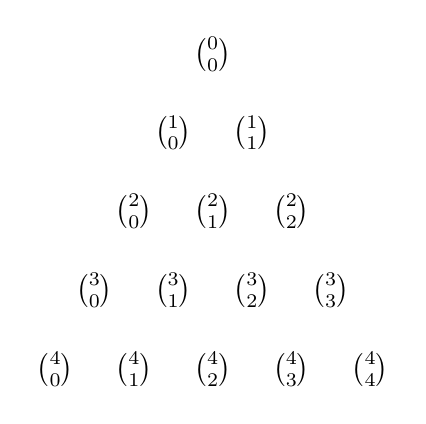
\begin{tikzpicture}
    \foreach \n in {0,...,4} {
        \foreach \k in {0,...,\n} {
	    \node at (\k-\n/2,-\n) {${\n \choose \k}$};
	}
    }
\end{tikzpicture}
\caption{Pascal'sches Dreieck bis zum Grad 4}
\end{figure}

